\section{Implementation}

\subsection{The end-to-end solution}

The lookalike model works on the hypothesis that sparse users belonging to the same cluster as predicted by our k-means model (trained on dense users) should exhibit similar interaction preferences. By taking this preference into consideration in our ranking, we should notice a better reward rate and higher engagement from our sparse users – eventually turning them into dense users. 

Our recommendation system would therefore consist of: 

\begin{itemize}
    \item Identifying the cluster number that a cold or sparse user belongs to 
    \item Fetching the associated weight vector for the categories of the content 
    \item Ranking the Bubbles by using this vector as the defining rubric 
\end{itemize}

For the sake of our experiment, we will test this A/B on a set of 400,000 active users. The architecture overview is provided in figure \ref{fig:arch}.

\begin{figure*}
  \centering
  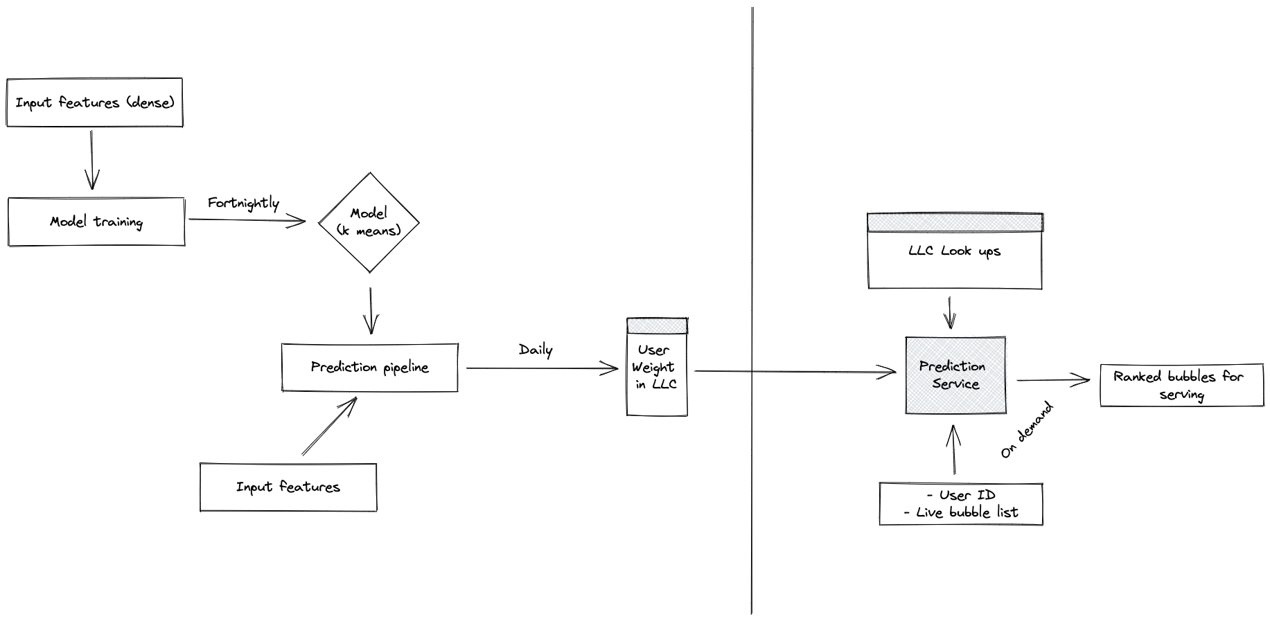
\includegraphics[width=\textwidth]{figures/arch.jpeg}
  \caption[Architecture diagram of the end-to-end system]{Overview of the end-to-end system design}
  \label{fig:arch}
\end{figure*}

\subsection{Specification of the prediction service}

Our recommendation systems at Glance operate under some tight constraints: 

\begin{itemize}
    \item Latency of the prediction model should be less than 150ms 
    \item The number of Bubbles ranked per user request can go up to 400 Bubbles per request 
    \item At any given time, we have roughly 4000 content pieces in our repository to be served, as they keep getting refreshed. 
\end{itemize}

We have one pipeline to train our clustering model on our dense users. We do not expect a lot of drift in the data, so this model could be refreshed as lazily as every fortnight. The users belong to our control subset, so that other model biases are not introduced into the dataset. This subset forms 10\% of our active user base, which has a very simple serving algorithm which we will compare ourselves with, called {\itshape Pacing}. 

A second pipeline runs at a daily cadence, to identify the cluster number of the users in our experiment. This pipeline loads the k-means model and runs clustering on target set of users. It then uses the weight matrix to identify the corresponding category weights for the user. The {\verb|[user_id, category_weight]|} mapping is saved in a low latency cache. This pipeline takes about 7 minutes to run. 

Our prediction service takes three inputs:  
\begin{itemize}
    \item {\verb|user_id|}: a unique identifier for the user in our system  
    \item {\verb|bubble_count|}: number of Bubbles to be ranked 
    \item and {\verb|live_bubbles|}: a candidate list of Bubbles to rank 
\end{itemize}

It fetches the {\verb|category_weight|} of the user from the low latency cache. It then looks up two attributes for every Bubble in {\verb|live_bubbles|}: category and global popularity of the Bubble. The global popularity of a Bubble is sampled from a beta distribution composed of the positive and negative interactions of the users on that Bubble, over a period of the previous 30 days. All the lookups are locally cached to avoid repeated network calls. 

The {\verb|category_weight|} of a user identifies a category affinity. We need to translate this to a Bubble level score. To do that we envision {\verb|bubble_count|} number of slots to fill with {\verb|live_bubbles|}. The {\verb|category_weight|} tells us which category the user is more likely to interact with. Multinomial sampling with the different categories weighed differently lets us divide bubble count into category slots. A category slot is filled in with the most popular bubble in the live bubbles list, according to global popularity score. 

The category weight only tells how likely a cluster is to interact with the categories and should not be interpreted as order of interaction. Say “fashion” had 0.5 and “sports” had 0.3 as their category weights for a certain cluster. This doesn't mean fashion content should come "first" while ranking the content, all this means is that fashion was preferred more as a category. Therefore, we do not encode the category weight into the final score associated with the Bubble and use it only to dictate the number of Bubbles. The popularity score serves as the final step to attach a score to every bubble. 

Two further tweaks make this ready for production: 
\begin{itemize}
    \item A 20\% reservation to explore categories uniformly, to better identify category affinity
    \begin{itemize}
        \item Essentially our model operates on 80\% of {\verb|bubble_count|}, with 20\% of the {\verb|bubble_count|} sampled from a uniform distribution of category weights 
    \end{itemize}
    \item A fallback mechanism for when {\verb|category_weight|} is unavailable for a user
    \begin{itemize}
        \item Because the pipeline runs at a daily cadence there would be users who would not be touched by the pipeline yet, and hence have no {\verb|category_weight|}. For such users we fallback to scoring the bubbles basis their global popularity, sampling from the global interaction distribution. 
    \end{itemize}
\end{itemize}

Because the final prediction service does only light weight calculations it is extremely fast. It can maintain a steady state p99 latency of 60ms. 

\begin{figure}[h]
  \centering
  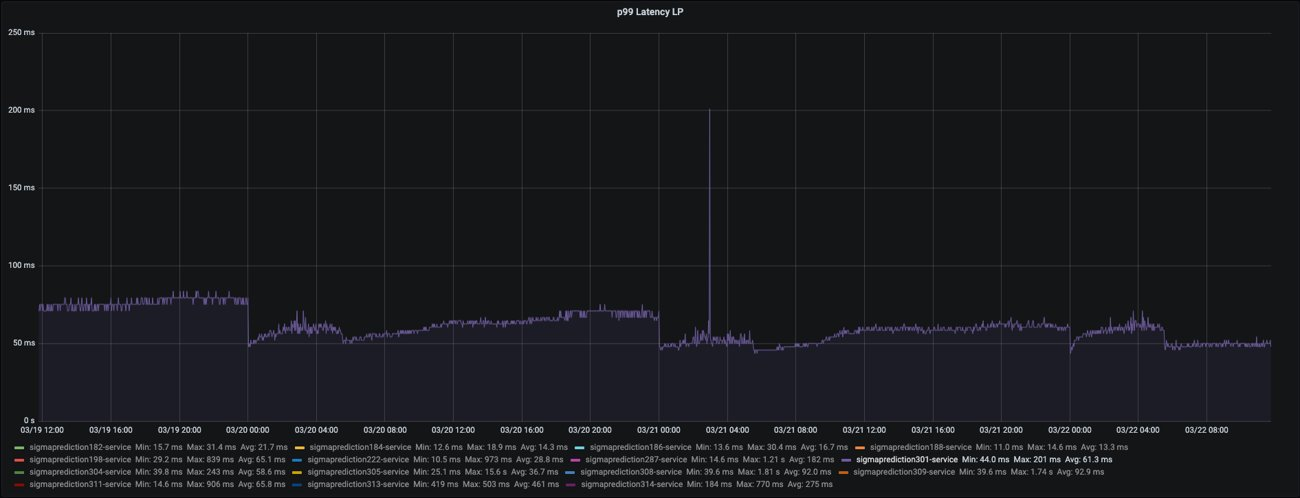
\includegraphics[width=\linewidth]{figures/latency.jpeg}
  \caption[P99 Latency of the prediction service]{Grafana dashboard showing the p99 latency of the prediction service, at a steady state of around 60ms}
  \label{fig:latency}
\end{figure}

